%!TEX encoding = UTF-8 Unicode
%!TEX TS-program = pdflatex

%%% --- PREAMBLE --- %%%
\documentclass[a4paper,11pt]{article}

\usepackage[italian]{babel}
\usepackage[left=2cm,right=2cm,top=2cm,bottom=2cm,headheight=14pt]{geometry}
\usepackage[T1]{fontenc} % OT1: basic, T1: western, T3 and T5: exotic, T4: lots of characters but WORSE READABILITY
\usepackage[utf8x]{inputenc} % utf8x supports more characters than utf8
\usepackage{graphicx} % import PNG, JPG and PDF with \includegraphics
\usepackage[usenames,table]{xcolor} % \color
\usepackage{amssymb}
\usepackage{amsmath}
\usepackage{amsfonts}
\usepackage{float}
\usepackage{mathtools} % (!! PLACE BEFORE hyperref !!)
\usepackage{xfrac} % \sfrac
\usepackage{cancel} % \cancel \cancelto
\usepackage{hyperref} % interactive links in TOC, URLs and references
% unneded \usepackage{fixltx2e} % provides \textsubscript and makes some fixes
\usepackage[toc,page]{appendix}
\usepackage{siunitx} % \num \si \SI
\usepackage{alltt} % {alltt} (like verbatim but with commands)
\usepackage{moreverb} % {listing}
\usepackage{listings} % {lstlisting}
\usepackage[overload]{textcase} % fixes \MakeUppercase and \MakeLowercase
\usepackage[normalem]{ulem} % \uline \uwave \sout \xout
\usepackage{enumerate} % adds options for {enumerate}
\usepackage{paralist} % inline lists with {inparaenum}
\usepackage[official]{eurosym} % \euro
\usepackage{tabu} % {tabu} (like {tabular} with improvements)
\usepackage{layout} % layout description
\usepackage{multicol} % {multicols}
\usepackage{lipsum} % filling text generator with \lipsum
\usepackage[section]{placeins} % inhibits float figures from trepassing a section boundary
\usepackage{subfig} % \subfloat to be used inside {figure}
\usepackage{wrapfig} % {wrapfigure} (like {figure} but allows text to flow on its sides)
\usepackage{ifthen} % \ifthenelse
\usepackage{calc}
\usepackage{array}
\usepackage{multirow}
\usepackage{booktabs} % \toprule, \midrule, \bottomrule
\usepackage{fancyhdr}
\usepackage{wasysym}
\graphicspath{ {../Figs-Tabs/} } % graphics search directories
\setcounter{tocdepth}{1} % -1: part, 0: chapter, 1: section, 2: subsection, 3: subsubsection

\lstset{ %
	language=C,
	deletekeywords={},
	morekeywords={},
	backgroundcolor=\color{white},
	basicstyle=\ttfamily\small,
	commentstyle=\color{teal},
	keywordstyle=\color{magenta},
	stringstyle=\color{purple},
	identifierstyle=\color{violet!80!black},
	numbers=left,
	numbersep=7pt,
	numberstyle=\scriptsize\sffamily\color{gray},
	stepnumber=1,
	breakatwhitespace=false,
	breaklines=true,
	keepspaces=true,
	showspaces=false,
	showstringspaces=false,
	showtabs=false,
	tabsize=2,
	captionpos=none,
}

\newcommand{\ndr}[1]{\footnote{#1 (n.d.r.)}}

\newcommand{\fig}[1]{\figurename{ \ref{fig:#1}}} %inserting reference to figures
\newcommand{\tab}[1]{\tablename{ \ref{tab:#1}}} % inserting reference to tables
\newcommand{\eqn}[1]{equazione \eqref{eq:#1}} % inserting reference to equation

\newcommand{\dof}{\text{ dof}} % degrees of freedom
\newcommand{\paral}{\mathbin{\|}} % impedance parallel
\DeclareSIUnit\deca{decade} % decade unit definition for use in siunitx
\DeclareSIUnit\gauss{Gs} % Gauss unit definition for use in siunitx

\newcommand{\insertpart}[2]{\input{#1}}
\newcommand{\e}{\textbf{$e^{-}$}}

\sisetup{%
	separate-uncertainty = true,
	per-mode = symbol,
	bracket-numbers = false,
	multi-part-units = single,
	table-number-alignment = center,
	range-phrase = \text{--},
	range-units = single,
	output-complex-root =  \text{\ensuremath{j}},
	table-figures-decimal = 3,
	table-figures-exponent = 0,
	table-figures-integer = 2,
	table-figures-uncertainty = 2,
}

%%% --- DOCUMENT --- %%%


%%%%% SIunits example use:
% \si{\kilo\volt\per\meter\squared} -> kV/m^2
% \SI{1.222 (34)}{\joule\second}    -> 1.222 +- 0.034 Js
% \SI{1.222 \pm 0.034}{\nF}         -> 1.222 +- 0.034 nF
% use it plz

\pagestyle{fancy}
\author{Gruppo BF \\ Thomas Giannoni, Valerio Lomanto, Roberto Ribatti}
\title{Esercitazione N. 13: Macchine a stati finiti: semaforo }
\date{2 maggio 2017}

\begin{document}
\maketitle
\begin{abstract}
In quest'esperienza sono state realizzate  alcune macchine a stati finiti (FSM) che
gestiscono un semaforo.
Le prime due macchine finite ivi riportate sono state realizzate con circuiti integrati;
basandole su Flip-Flop D-Latch. La prima di esse implementa un semaforo costantemente abilitato,
che alterni gli stati :

Verde acceso $\longrightarrow$ Verde e
giallo acceso $\longrightarrow$ rosso acceso $\longrightarrow$
verde acceso  ciclicamente.

La seconda FSM realizzata con
circuiti integrati riprende la precedente introducendo un segnale di abilitazione;
con il semaforo disabilitato sono stati imposti gli stati:

Led giallo acceso $\leftrightarrow$ Led giallo spento.

Nella seconda fase dell'esperienza è stato realizzato un programma che attraverso ARDUINO
implementi il semaforo abilitabile.
\end{abstract}
\section{Strumentazione}
	In qest'esperienza esperienza sono stati impiegati :
	\begin{itemize}
		\item 2 circiti integrati SN7400 usati per costituire i circuiti in esame
		\item varie resistenze e capacità impiegate anch'esse per il montaggio dei circiti
		\item 1 DIP switch a 4 interruttori
		\item 1 diodo 1N418
		\item 2 diodi LED, impiegati per rendere osservabile visivamente le tabelle di verità. 
		\item Il circito impulsatore basato sul Arduino nano montato nell'esperienza n.10
		\item un multimetro digitale
		\item un oscilloscopio digitale 
		\item un generatore di funzioni d'onda
	\end{itemize}

\section{verifica tabella NEND}
	Per la verifica della tabella di verità di una porta NEND 
	\tablename{
		 \ref{t:NEND}
	 }
	si è proceduto in due maniere distinte. Una prima verifica visiva, che impieghi il DIP SWITCH in dotazione; 
	ed una che impieghi il circuito impulsatore basato su arduino.
	Per entrambi i modi si è montato il circuito in \figurename{ \ref{f:NEND}}.
	In tale circuito si è 
	impiegata una resistenza di pull-ups $R_{Pull-ups}=$\SI{983	\pm 8	}{\ohm} per migliorare 
	l'operatività del circito;
	una resistenza $R_{1}=$\SI{330 \pm 3 }{\ohm} montata per  limitare la richiesta di corrente al diodo.
	Il diodo LED D1 è posto in serie con $R_{1}$ e chiuso su GROUND.
	L'integrato  SN7400 è stato alimentato con una tensione di alimentazione $V_{cc}=$\SI{ 5.01 \pm 0.03  }{\volt}.
	\begin{figure}[htb]
		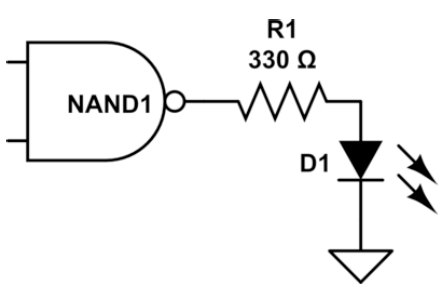
\includegraphics[scale=0.35]{../Figs-Tabs/NEND.png}
	\end{figure}\label{f:NEND}

\begin{table}[htb]
	\centering
	\begin{tabular}{sss}
		\toprule
		\text{ingresso} A & \text{ingresso} B &\text{uscita porta NAND }$\overline{A\cdot B}$	\\
		\midrule
		0  & 0 & 1\\
		0  & 1 & 1\\
		1  & 0 & 1\\
		1  & 1 & 0\\
		\bottomrule
	\end{tabular}
	\caption{Tabella di verità di una porta NEND.}
	\label{t:NEND}
\end{table}

\subsection{osservazione con dip switch}
	Essendo le porte NAND impiegate basate su logica TTL quando esse non risultino collegate a terra si ottiene in uscita un segnale corrispondente allo stato HIGH; cosa che non avviene qualora si abbia un collegamento a terra.
	Si è pertanto procedto a collegare da un lato gli ingressi 1 e 2 del deap switch alla tensione di GROND e da l'altro rispettivamente agli ingressi A e B del NEND.
	
	Il diodo led  essendo acceso qalora l'uscita del NEND sia alta
	e spento qualora  l'uscita sia in stato LOW
	permette la verifica della tabella di verità.
	
	Si è procedto pertanto alla verifica della tabella di verità provando le varie permitazioni degli switch 1 e 2, ottenendo n perfetto accordo con \tablename{ \ref{t:NEND}}.
\subsection{Impiego di Ardino e del oscilloscopio}\label{sez:ard}
	Per effettare una ulteriore verifica di tale tabella di verità 
	si è proceduto a collegare le porte A e B della porta NAND rispettivamente alle 
	uscite Y1 ed Y2 del circuito impulsatore, realizzato con arduino nell'esperienza 10,
	e si  collegata l'uscita della NAND all'oscilloscopio.
	
	Essendo le traccie ottente alle porte Y1 e Y2 dell'impulsatore due onde quadre 
	sfasate relativamente di $\pi/2$ su di un periodo assumono tuttue le permutazioni di due ingressi ad un bit.
	Si riportano le acquisizioni ottente all'oscilloscopio in \figurename{ \ref{f:osci}} .
	\begin{figure}[hb]
		\centering
		\subfloat[acquisizione delle tensioni in ingresso nella porta NEND; A (ch1) ed B (ch2)]{
		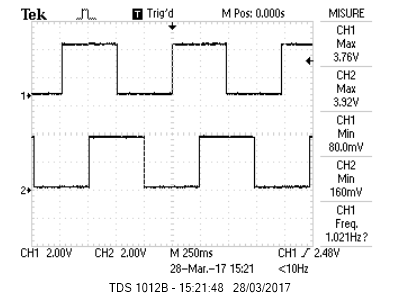
\includegraphics[scale=0.35]{../Figs-Tabs/ingressi.png}
		\label{f:ing}
	}\\
	\subfloat[acquisizione uscita porta NEND (ch2) e della tensione in ingresso A (ch1)]{
		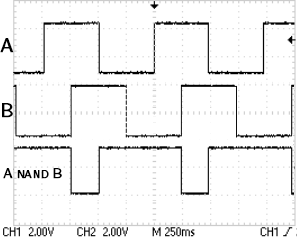
\includegraphics[scale=0.35]{../Figs-Tabs/NAND.png}
		\label{f:sci}
	}\\
	\caption{acquisizioni delle schermate impiegate per la verifica di \tablename{ \ref{t:NEND}}.}
	\label{f:osci}
\end{figure}

	Per rendere significativa l'acquisizione dell'uscita dalla porta NEND ( \figurename{ \ref{f:sci}} ) si è acquisito contemporaneamente uno dei de ingressi, nella fattispecie A; dopodiché si sono acquisiti entrambi i segnali  in ingresso (\figurename{ \ref{f:ing}} ) quale indicazione dello stato di ingresso.
	
	Dall'osservazione della \figurename{ \ref{f:osci}} si ottiene un ulteriore verifica della \tablename{ \ref{t:NEND}}.
\section{Progettazione e verifica semplici circiti logici}
	Per verificare le tabelle di verità dei seguenti circuiti si è impiegato il circuito impulsatore; ed in particolare la tecnica descritta in\textbf{ sezione \ref{sez:ard} }.
	Si segnala che per tutta la sezione verrà impiegata la \figurename{ \ref{f:ing}} quale riferimento per i segnali in ingresso.
	\subsection{AND}
	Per verificare l'andamento di un circuito AND, essendo
	$$AND(A,B) = A \cdot B = \overline{(\overline{A \cdot B})}$$
	si è montato il circuito in \figurename{ \ref{f:AND}} 
	\begin{figure}[htb]
		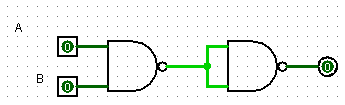
\includegraphics[scale=1.0]{../Figs-Tabs/ENd.png}
		\caption{rappresentazione di un circito AND realizzato con porte NAND. A e B rappresentano gli ingressi mentre si campiona in scita sl terzo terminale.}
	\end{figure}\label{f:AND}
.
	Tale circito presenta la tabella di verità riportata in \tablename{ \ref{t:AND}} 
	\begin{table}[htb]
		\centering
		\begin{tabular}{sss}
			\toprule
			\text{ingresso} A & \text{ingresso} B &\text{uscita porta AND }$A\cdot B$	\\
			\midrule
			0  & 0 & 0\\
			0  & 1 & 0\\
			1  & 0 & 0\\
			1  & 1 & 1\\
			\bottomrule
		\end{tabular}
		\caption{Tabella di verità di una porta AND.}
		\label{t:AND}
	\end{table}.
	la quale risulta a sua volta verificata dall'andamento osservato
	e riportato in \figurename{ \ref{f:osci-and}}
	
	\begin{figure}[hb]
		\centering
		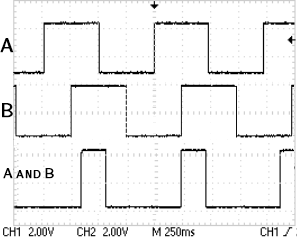
\includegraphics[scale=0.35]{../Figs-Tabs/and.png}
		\caption{acqusizione della schermata impiegata per la verifica di \tablename{ \ref{t:AND}}.
		Uscita funzione AND (ch2) e tensione in ingresso in A (ch1).
		}
		\label{f:osci-and}
	\end{figure}.
	\subsection{OR}
			Per la funzione OR essendo $$ OR(A,B) = A + B = \overline{\overline{(A +B)}}= \overline{(\overline{A} \cdot \overline{B})}$$
			è stato montato il circuito in \figurename{ \ref{f:OR}} 
		\begin{figure}[htb]
			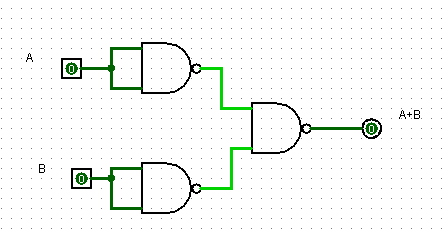
\includegraphics[scale=1.0]{../Figs-Tabs/OR2.png}
			\caption{rappresentazione di un circito OR realizzato con porte NAND. A e B rappresentano gli ingressi mentre si campiona in uscita sul terzo terminale.}
		\end{figure}\label{f:OR}.
		Tale circito presenta la tabella di verità riportata in \tablename{ \ref{t:OR}} 
		\begin{table}[htb]
			\centering
			\begin{tabular}{sss}
				\toprule
				\text{ingresso} A & \text{ingresso} B &\text{uscita porta AND }$A\cdot B$	\\
				\midrule
				0  & 0 & 0\\
				0  & 1 & 1\\
				1  & 0 & 1\\
				1  & 1 & 1\\
				\bottomrule
			\end{tabular}
			\caption{Tabella di verità di un circito OR.}
			\label{t:OR}
		\end{table}.
		la quale risulta a sua volta verificata dall'andamento osservato
		e riportato in \figurename{ \ref{f:osci-or}}
		
		\begin{figure}[hb]
			\centering
			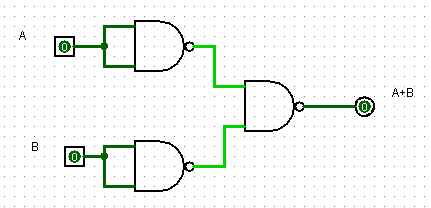
\includegraphics[scale=0.35]{../Figs-Tabs/or.png}
			\caption{acquisizione della schermata impiegata per la verifica di \tablename{ \ref{t:OR}}.
				Uscita circito OR (ch2) e tensione in ingresso in A (ch1).
			}
			\label{f:osci-or}
		\end{figure}.
	\subsection{XOR}
	Per la funzione XOR essendo $$ XOR(A,B) = A \oplus B = (A \cdot \overline{B}) + (\overline{A} \cdot B) =
	 \overline{
	 	\overline{
	 		( A \cdot \overline{
	 			(A \cdot B) )
 			}	\cdot 
 		\overline{
 			(B \cdot \overline{
 				(A \cdot B)
 			} )
 		}
 	}
	}$$
	è stato montato il circuito in \figurename{ \ref{f:XOR}} 
	\begin{figure}[htb]
		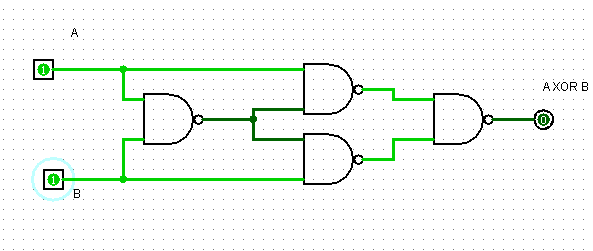
\includegraphics[scale=1.0]{../Figs-Tabs/XOR2.png}
		\caption{rappresentazione di un circuito XOR realizzato con porte NAND. A e B rappresentano gli ingressi mentre si campiona in uscita sul terzo terminale.}
	\end{figure}\label{f:XOR}.
	Tale circuito presenta la tabella di verità riportata in \tablename{ \ref{t:XOR}} 
	\begin{table}[htb]
		\centering
		\begin{tabular}{sss}
			\toprule
			\text{ingresso} A & \text{ingresso} B &\text{uscita porta XOR }$A \oplus B$	\\
			\midrule
			0  & 0 & 0\\
			0  & 1 & 1\\
			1  & 0 & 1\\
			1  & 1 & 0\\
			\bottomrule
		\end{tabular}
		\caption{Tabella di verità di un circito XOR.}
		\label{t:XOR}
	\end{table}.
	la quale risulta a sua volta verificata dall'andamento osservato
	e riportato in \figurename{ \ref{f:osci-xor}}
	
	\begin{figure}[hb]
		\centering
		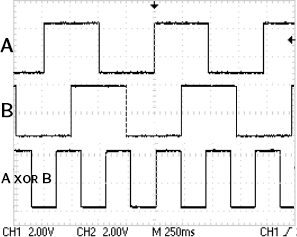
\includegraphics[scale=0.35]{../Figs-Tabs/xor.png}
		\caption{acqusizione della schermata impiegata per la verifica di \tablename{ \ref{t:XOR}}.
			Uscita circito XOR (ch2); tensione in ingresso in A (ch1).
		}
		\label{f:osci-xor}
	\end{figure}.
\subsection{Circito sommatore ad un bit}	
	Per realizzare il circuito sommatore richiesto si è assunto
	che esso potesse costituirsi su un uscita [uscita 1] di una funzione XOR, per esprimere il bit più significativo;
	ed da una funzione AND sull uscita rimanente [uscita 2] per esprimere il meno significativo.
	Si è montato pertantonto il circito in \figurename{ \ref{f:somma}}.
		\begin{figure}[htb]
		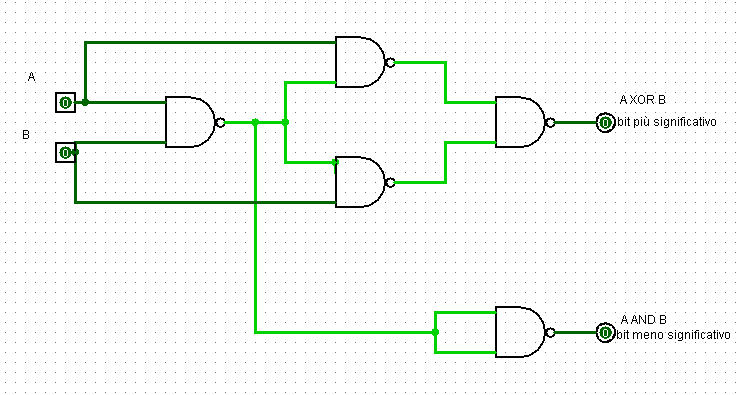
\includegraphics[scale=1.0]{../Figs-Tabs/somma.png}
		\caption{rappresentazione di un circito sommatore a 2 ingressi e 2 uscite.}
	\end{figure}\label{f:somma}
	
	L'andamento del circito risulta verificato dalla 	\figurename{ \ref{f:osci-somma}}.
	
	\begin{figure}[hb]
	\centering
	\subfloat[acqsizione della tensione in uscita dal circito XOR (ch2) ed in ingresso A (ch1);
	tale figura costituisce insieme alla \figurename{ \ref{f:ing}} un riferimento]{
		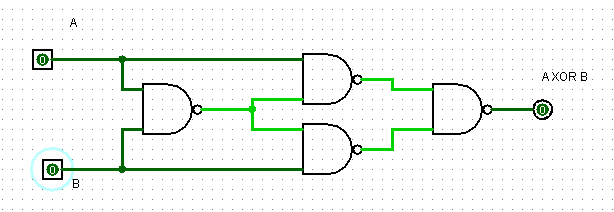
\includegraphics[scale=0.35]{../Figs-Tabs/XOR.png}
		\label{f:ing-somma}
	}\\
	\subfloat[acquisizione delle tensioni in uscita dal circito XOR (ch2) ed in uscita dal circito AND (ch1)]{
		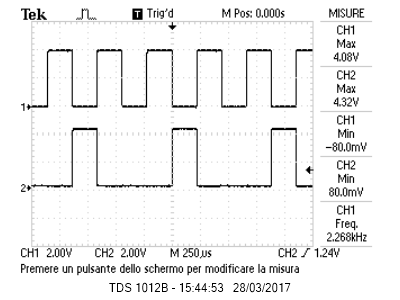
\includegraphics[scale=0.35]{../Figs-Tabs/sommatore_out.png}
		\label{f:sci-somma}
	}\\
	\caption{acqusizioni delle schermate impiegate per la verifica del funzionamento del circuito sommatore.}
	\label{f:osci-somma}
\end{figure}
Si può infatti osservare che l'uscita assuma alternativamente i valori $00-01-10-11$.


\section{Generatore di onda quadra}
	Per la realizzazione di un generatore di onda quadra
	si sono impiegati i circuiti impiegati per il multivibratore monostabile e
	per il multivibratore astabile 
	accoppiandoli in maniera da ottenere il da ottenere il circuito in \figurename{ \ref{f:qadra}}.
	\begin{figure}[htb]
		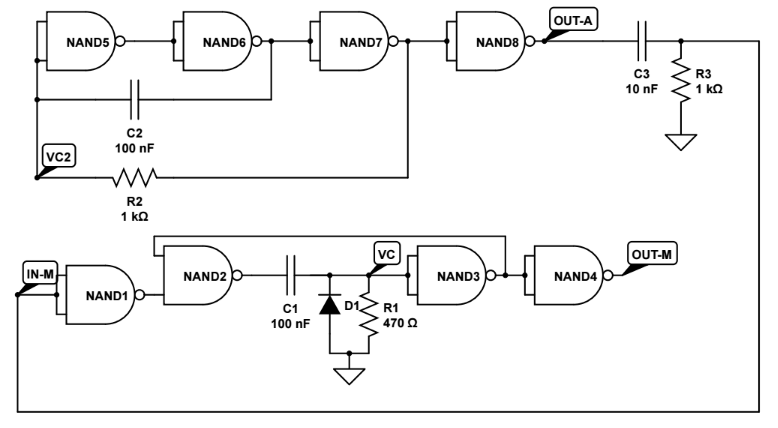
\includegraphics[scale=1.0]{../Figs-Tabs/qadra.png}
		\caption{rappresentazione del circuito realizzato per generare un onda quadra.}
	\end{figure}\label{f:qadra}

	Per il montaggio circuitale sono state impiegate le seguenti componenti\footnote{Tali valori sono stati ottenuti attraverso il multimetro digitale in dotazione. A tali misure sono state associate le incertezze calcolate sommando in quadratura l'errore di lettura con l'errore di calibrazione dello strumento.} :\\
	\begin{center}
		$R_{3}=$\SI{988 \pm 8}{\ohm}\\
		$C_{3}=$\SI{10.8 \pm 0.4 }{\nano \farad}\\
	\end{center}
	
	Si riportano in \figurename{ \ref{f:osci-qad}} l'acquisizione del segnale in 
	ingresso nel multivibratore monostabile; ovvero il segnale in uscita dal derivatore (ch2) ed il segnale in ingresso (ch1).
	\begin{figure}[htb]
		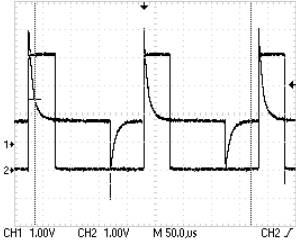
\includegraphics[scale=1.0]{../Figs-Tabs/deth_generator.png}
		\caption{Acquisizione dei segnali in ingresso [ch1] ed in uscita [ch2] dal circuito monostabile.}
	\end{figure}\label{f:osci-qad}
	Il circuito monostabile, come riscontrabile in \figurename{ \ref{f:osci-qad}},
	trasforma l'onda quadra generata dall'astabile in un impulso di breve durata temporale; sempre dalla figura in esame può essere osservato che il monostabile risulti sensibile al fronte di salita del segnale in ingresso.
	
	Come atteso, dall'andamento osservato in sezione 2, in uscita al circuito monostabile si ottiene un onda quadra [ch2 di \figurename{ \ref{f:osci-qad}}].
	Tale onda presenta un periodo 
	$T=$\SI{205 \pm 1 }{\mu \sec}
	\footnote{valori misurati con i cursori dell'oscilloscopio. Si è associata l'incertezza dovuta all'errore di posizionamento dei cursori; a cui si aggiunge a parte l'errore di calibrazione dello strumento.}
	a fronte di un impulso di $\Delta T_{up} =$\SI{47.0 \pm 0.2 }{\mu \sec}
	\footnote[1]{}
	Si ottiene pertanto un duty-cycle $\frac{\Delta T_{up}}{T}= 22.9 \pm 0.2$\textdiscount.
	
	Nella sezione 2 è stato osservato che l'impulso ,$\Delta T_{up}$, 
	abbia una dipendenza lineare dal valore della resistenza $R_{2}$;
	la durata del periodo ne risulti indipendente; poiché non varia apprezzabilmente al variare di $R_{2}$.
	
	Mentre nella sezione  è stata osservata la dipendenza lineare 
	del periodo $T$ dal valore della resistenza $R_{1}$;
	mentre la durata del impulso non vari significativamente.
	
	Si assume pertanto che $$ \Delta T_{up} \propto R_{2}$$
		$$T \propto R_{1} $$
	e non il viceversa.
	Per la verifica di tale assunzione si è proceduto a variare separatamente i valori di $R_{1}$ e $R_{2}$; si ottengono i dati in \tablename{ \ref{t:4}}.
		
	\begin{table}[htb]
		\centering
		\begin{tabular}{*{5}{S}}
			\toprule
			$R_{1}$ [\si{\ohm}] & $R_{2}$ [\si{\kilo \ohm}] & $T$ [\si{\mu \sec}] & $\Delta T_{up}$  [\si{\mu \sec}] & $\frac{\Delta T_{up}}{T}$ \\
			\midrule
			470\pm 5	&	1.12 \pm 0.01	&	234 \pm 1	&	47.6\pm2	&	4.92 \pm3	\\ 
			567 \pm6	&	1.12 \pm 0.01	&	234\pm1	&	59.2 \pm4	&	3.95\pm 0.03	\\ 
			567 \pm6	&	0.988 \pm 0.009	&	205\pm1	&	59.2 \pm0.4	&	3.46\pm0.03	\\ 
			\bottomrule
		\end{tabular}
		\caption{
			Tabella dei valori campionati per la verifica delle dipendenze di $\Delta T_{up}$ e $T$ dai valori di $R_{1}$ e  $R_{2}$.
		}
		\label{t:4}
	\end{table}
	Come possiamo osservare dai valori tabulati si ottiene un sostanziale accordo con la proporzionalità attesa.
	
	Si è adesso proceduto a realizzare un generatore di onde quadre di $T_{att}\sim 100$\si{\mu \sec} e $ \Delta {T_{up}}_{att}\sim 30$\si{\mu \sec}.
	
	Dai valori ottenuti nelle sezioni 2 e 3 e  dai rispettivi coefficienti stimati $a=$ e $b=$
		abbiamo stimato per i valori richiesti delle resistenze attese 
	${R_{2}}_{att}=$\SI{470 \pm 30}{\ohm}%valore placeholder
	${R_{1}}_{att}=$\SI{260 \pm 40}{\ohm}%valore placeholder.
	Si è osservato tuttavia che impiegando tali resistori si ottiene un impulso sensibilmente diverso da quello atteso.
	Si è pertanto proceduto a variare i valori delle resistenze sino ad ottenere un accordo tra i valori misurati e quanto richiesto.
	Al termine di tale processo sono state impiegate delle resistenze 
	$R_{1}=$\SI{331 \pm 3}{\ohm}
	$R_{2}=$\SI{464 \pm 4}{\ohm}
	ottenendo 
	$T=$\SI{101 \pm 1}{\mu \sec} e $ \Delta {T_{up}}=$\SI{30.2 \pm 0.2}{\mu \sec}.
	
	Una posssibile causa della discrepanza tra i valori dei resistori, per cui si verifichi l'accordo con le richieste, ed  i valori di ${R_{2}}_{att}$ e 	${R_{1}}_{att}$ potrebbe essere imputabile ad un andamento non esattamente lineare nelle dipendenze di $ \Delta T_{up}$ da $ R_{2}$ e di
	$T $ da $ R_{1} $
	
	
	
	
	
	
	
	
	
	

\paragraph{Semaforo privo di enable}
Per la realizzazione una FSM che alterni gli stati come in \figurename{\ref{fig:stati}}
Avendo tre stati diversi è stato necessario impiegare una codifica a 2 bit.
Essendo la codifica arbitraria si riporta la codifica impiegata in 
\tablename{\ref{tab:cod}}.
Essendo possibile con due bit ottenere anche lo stato $00$,  non corrispondente a nessuno degli stati codificati,
è stato imposto che dallo stato $01$ sul successivo fronte di salita di clock il segnale costituisca
la transizione \\VERDE E GIALLO $(0;1)$  $\longrightarrow$ ROSSO $(1;0)$.
Rendendo pertanto il lo stato $0;0$ inaccessibile.
Si riporta la \tablename{ \ref{tab:tran}} delle transizioni tra i vari stati della FSM.
Per la progettazione della macchina è stata impiegata la codifica di Mealy così da minimizzare il numero di porte logiche impiegate.
Dalla \tablename{ \ref{tab:tran}} si ottiene  $b_{1}^{n+1} =  \overline{b_{1}^{n} \cdot b_{0}^{n}}$ e $b_{0}^{n+1} = b_{1}^{n}$

Per realizzare la FSM basata sugli integrati a disposizione, e che realizzi quanto appena descritto,
 è stato realizzato il circuito in \figurename{ \ref{fig:sem2}} alimentando la componentistica con una tensione 
 $V_{cc}\sim 5$\si{\volt}.Si segnala inoltre che in serie con i led sono state montate delle resistenze $R\sim 330$\si{\ohm} per limitare la richiesta di corrente dei diodi LED.
\begin{figure}[h!]
	\begin{minipage}{0.5\textwidth}
		\centering
		\includegraphics[scale=0.20]{immagine.png}
		\caption{Stati della FSM semaforo senza En.}
		\label{fig:stati}
	\end{minipage}
\begin{minipage}{0.5\textwidth}
	\centering
	\begin{tabular}{ssc}
	\toprule
	b_{0} & b_{1} & stato corrispondente\\
	\midrule
	1 & 1 & VERDE\\
	0 & 1 & GIALLO \& VERDE\\
	1 & 0 & ROSSO\\
	0 & 0 &  X (NON VOLUTO)\\
	\bottomrule
	\end{tabular}
	\caption{Codifica degli stati impiegati}
	\label{tab:cod}
\end{minipage}
\end{figure}


\begin{table}[h]
\centering
\begin{tabular}{ss|ss|sss}
	\toprule
	b_{1}^{n} & b_{0}^{n}  & b_{1}^{n+1} & b_{0}^{n+1} & \text{LED VERDE} & \text{LED GIALLO} & \text{LED ROSSO} \\
	\midrule
	 0 & 0 & 0 & 1  & x  & x & x \\
	 0 & 1 & 1 & 1  & 0 & 0 & 1  \\
	 1 & 1 & 1 & 0  & 1 & 0 & 0 \\
	 1 & 0 & 0 & 1  & 1 & 1 & 0 \\
	\bottomrule
\end{tabular}
\caption{Tabella delle transizioni della FSM semaforo sempre abilitato.
Il segnale $1$ corrisponde al LED acceso, $0$ LED spento.
Lo stato $b_{1}=0$ $b_{0}=0$ deve risultare inaccessibile. }
\label{tab:tran}
\end{table}

\begin{figure}[h!]
		\centering
		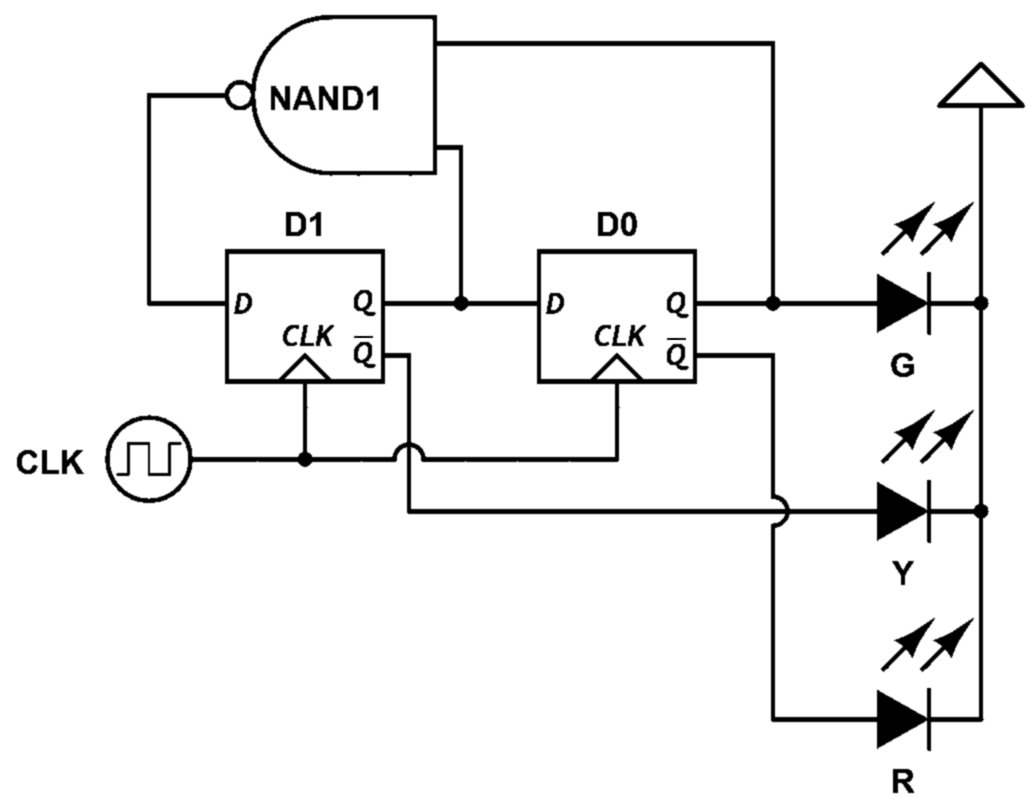
\includegraphics[scale=0.3]{circ3_.png}
		\caption{Circuito che realizzi il semaforo senza En.}
		\label{fig:sem2}
	\end{figure}

Per la verifica del funzionamento circuitale è stato 
 inviato un segnale di clock di frequenza bassa, $f<10 $\si{\hertz} e effettuando un primo controllo attraverso l'accensione dei LED. Si è successivamente aumentata la frequenza di clock $f= $\SI{175.937\pm 0.001}{\hertz}\footnote{Tale misura è stata presa con la funzione di acqusizione automatica dell'oscilloscopio;  l'incertezza associata è la prima cifra che risulti instabile.}
 ed acquisito i valori di tensione corrispondente alle uscite dei vari LED, riportate in 
 \figurename{ \ref{fig:acq}}. Dall'osservazione di
  tali acquisizioni si verifica l'accordo con le specifiche attese. 
 
\begin{figure}[h]
	\centering
	\subfloat[clock ch.1  LED VERDE ch. 2]{
		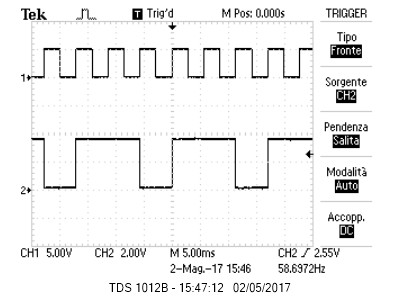
\includegraphics[scale=0.3]{./semaforosemplice/verde.jpg}
	}
	\subfloat[clock ch.1 LED GIALLO ch.2]{
		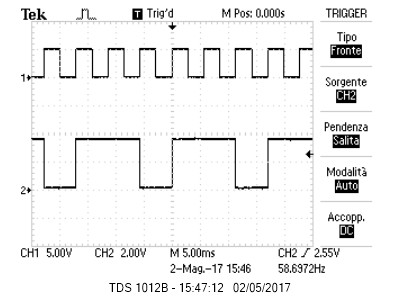
\includegraphics[scale=0.3]{./semaforosemplice/giallo.jpg}
		}\\
	\subfloat[clock ch.1  LED ROSSO ch.2]{
		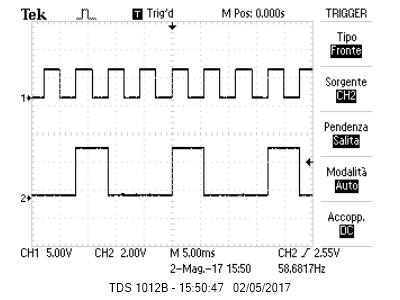
\includegraphics[scale=0.3]{./semaforosemplice/rosso.jpg}
		}
	\subfloat[clock ch.1  $b_{0}$ ch.2]{
		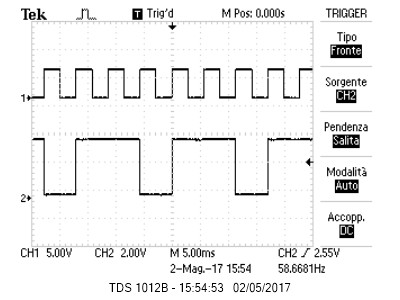
\includegraphics[scale=0.3]{./semaforosemplice/q-.jpg}
		}\\
	\subfloat[clock ch.1 $b_{1}$  ch.2]{
		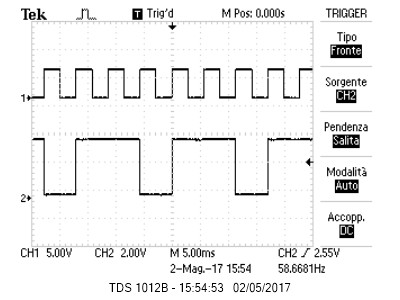
\includegraphics[scale=0.3]{./semaforosemplice/q+.jpg}
	}

	\subfloat[verde ch.1, giallo  ch.2]{
		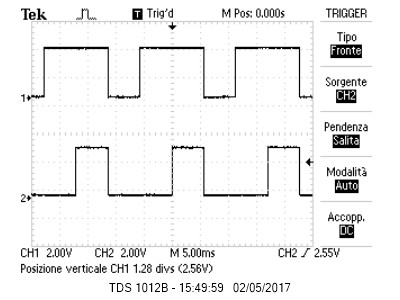
\includegraphics[scale=0.3]{./semaforosemplice/verde_giallo.jpg}
	}
	\subfloat[verde ch.1, rosso  ch.2]{
		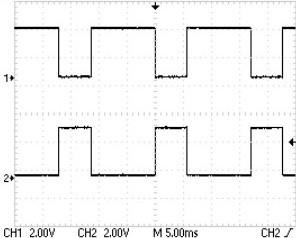
\includegraphics[scale=0.3]{./semaforosemplice/verde_rosso.jpg}
	}
\caption{Acquisizione telle tensioni osservate nel semaforo privo di ENABLE}
\label{fig:acq}
\end{figure}
\paragraph{Semaforo completo}
Per la realizzazione del semaforo completo si è proceduto ad implementare un ulteriore ingresso (En). Tale ingresso svolge la funzione di abilitare il circuito realizzato; in modalità abilitato il circuito realizzare deve comportare come descritto 
nella precedente sezione, mentre qualora si abbia il semaforo disabilitato devono alternarsi gli stati \\TUTTI LED SPENTI $\rightarrow$ LED GIALLO ACCESO ciclicamente.
Essendo arbitraria la codifica del valore di abilitazione è stato imposto che il semaforo sia abilitato
per $En = 1$; si è optato inoltre per realizzare un segnale di ENABLE sincrono; pertanto è stato aggiunto rispetto al 
circuito precedente un ulteriore FLIP-FLOP D-LEATCH.

Si riporta la  tabella di verita in \tablename{\ref{tab:tran2}}


\begin{table}[h]
	\centering
	\begin{tabular}{sss|ss|sss}
		\toprule
		b_{1}^{n} & b_{0}^{n} & En  & b_{1}^{n+1} & b_{0}^{n+1} & \text{LED VERDE} & \text{LED GIALLO} & \text{LED ROSSO} \\
		\midrule
		0 & 0 & 0& x & x & x & x& x\\
		0 & 0 & 1& 1 & 0 &  & & \\
		0 & 1 & 0& 1 & 1 &  & & \\
		0 & 1 & 1& 1 & 0 &  & & \\
		1 & 0 & 0& x & x &  & & \\
		1 & 0 & 1& 1 & 1 &  & & \\
		1 & 1 & 0& 0 & 1 &  & & \\
		1 & 1 & 1& 0 & 1 &  & & \\
		\bottomrule
	\end{tabular}
	\caption{Tabella delle transizioni della FSM semaforo completo.
		Il segnale $1$ corrisponde al LED acceso, $0$ LED spento.CONTROLLARE }
	\label{tab:tran2}
\end{table}

\end{document}
